\documentclass[aps,%
12pt,%
final,%
oneside,
onecolumn,%
superscriptaddress,%
centertags]{article} %%
\topmargin=10em
\textheight=600pt
\usepackage[english]{babel}
\usepackage[utf8]{inputenc}
\usepackage[colorlinks=true,urlcolor=black,linkcolor=black,filecolor=black,citecolor=black,unicode,pdftex]{hyperref}
%\usepackage{supertabular}
\usepackage[pdftex]{graphicx}
\usepackage{afterpage}
%\usepackage{amsthm,amssymb, amsmath}
%\usepackage{textcomp}
%\usepackage[noend]{algorithmic}
%\usepackage[ruled]{algorithm}

\selectlanguage{english}
\setlength{\parindent}{0cm}
\afterpage{\clearpage}

\newcommand{\compactlist}{\setlength{\itemsep}{0pt} \setlength{\parskip}{0pt} \setlength{\leftskip}{-1em}}

\renewcommand{\topfraction}{0.85}
\renewcommand{\textfraction}{0.1}
\renewcommand{\floatpagefraction}{0.75}

% See p.105 of "TeX Unbound" for suggested values.
% See pp. 199-200 of Lamport's "LaTeX" book for details.
%   General parameters, for ALL pages:
\renewcommand{\topfraction}{0.9}	% max fraction of floats at top
\renewcommand{\bottomfraction}{0.8}	% max fraction of floats at bottom
%   Parameters for TEXT pages (not float pages):
\setcounter{topnumber}{2}
\setcounter{bottomnumber}{2}
\setcounter{totalnumber}{4}     % 2 may work better
\setcounter{dbltopnumber}{2}    % for 2-column pages
\renewcommand{\dbltopfraction}{0.9}	% fit big float above 2-col. text
\renewcommand{\textfraction}{0.07}	% allow minimal text w. figs
%   Parameters for FLOAT pages (not text pages):
\renewcommand{\floatpagefraction}{0.7}	% require fuller float pages
% N.B.: floatpagefraction MUST be less than topfraction !!
\renewcommand{\dblfloatpagefraction}{0.7}	% require fuller float pages

\begin{document}

\begin{titlepage}
\begin{center}

% Title
\textbf{\LARGE Git –- Subversion Translation} \\[2.0cm]
\textbf{\Large Specification Draft} \\[3.0cm]

\textbf{Alexander Kitaev} \\[0.7cm]
\textbf{Dmitry Pavlenko} \\[0.7cm]
\textbf{Marc Strapetz} \\[0.7cm]
\textbf{Semen Vadishev} \\[0.7cm]

\end{center}
\end{titlepage}

\topmargin=-10pt
\setcounter{page}{2}

\newpage
\hrule
\tableofcontents

\newpage
\hrule
\section{Introduction}
% S.: Max: replace "layer" word by "color" -- git is green, svn is red.%
% git history graph - green color, svn - red, and here are examples...%
% Use "combined history graph" instead of "generalized history graph"%
\renewcommand{\figurename}{Diagram}
In this paper we introduce translation mechanism of basic concepts employed by Subversion and Git. \emph{Translator} is the server-side implementation of this mechanism.
\\\\
We use the notation of combined history to illustrate considered scenarios. The combined history consists of two layers:
\\\\
1. Subversion history layer. See diagram \ref{svn_layer}.
\begin{center}
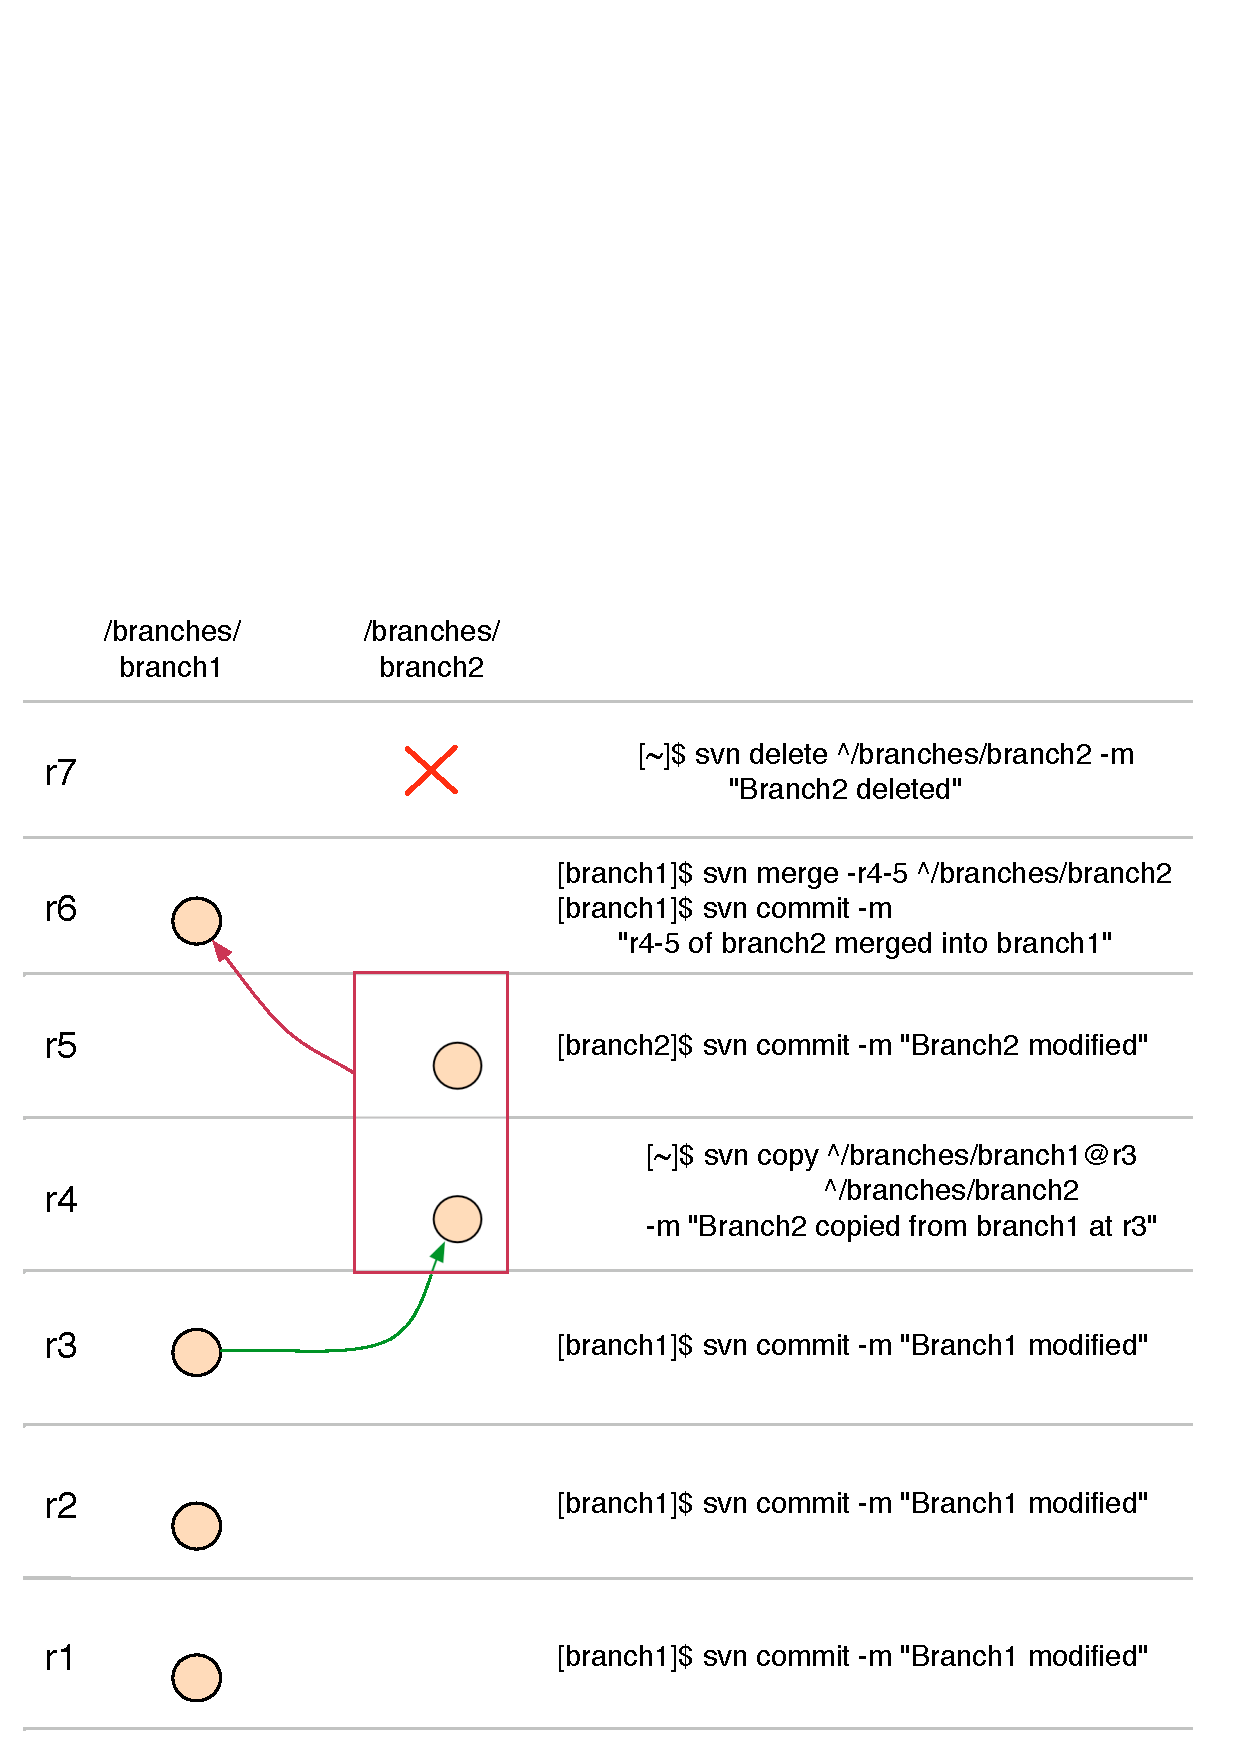
\includegraphics[width=\textwidth]{img/legend/svn_layer.pdf}%
\captionof{figure}{Subversion history layer.}
\label{svn_layer}%
\end{center}

2. Git history layer. See diagram \ref{git_layer}.
\begin{center}
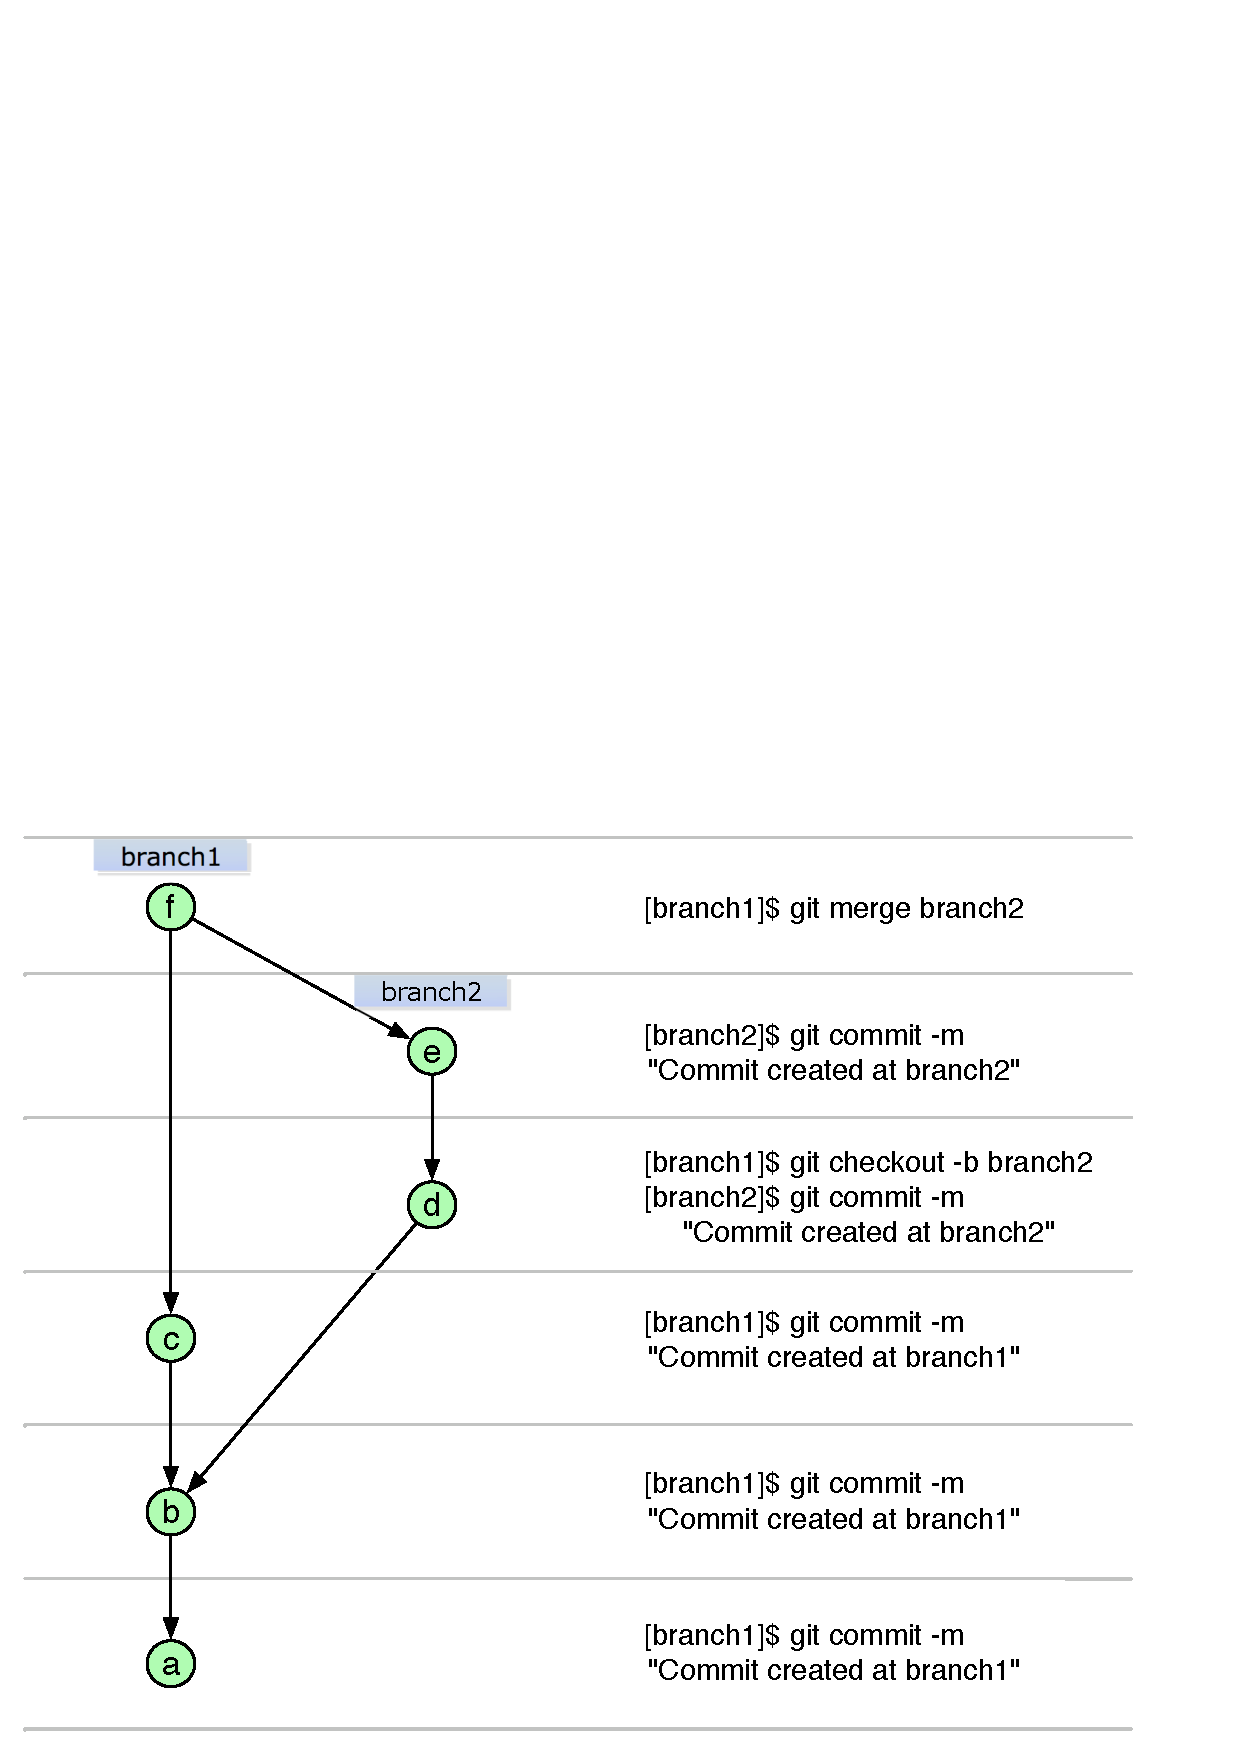
\includegraphics[width=\textwidth]{img/legend/git_layer.pdf}%
\captionof{figure}{Git history layer.}
\label{git_layer}%
\end{center}

First parent of merge commits will be always depicted as vertical arrow.
\\\\
To illustrate combined history we join described layers to put Git commits on top of corresponding SVN revisions as depicted at diagram \ref{both_layers}.
\begin{center}
\includegraphics[width=7.0cm]{img/legend/generalized_history.pdf}%
\captionof{figure}{Combined history.}
\label{both_layers}%
\end{center}

\newpage
\hrule
\section{Translator Architecture}
\subsection{Translator Components}
\renewcommand{\figurename}{Figure}

Translator runs as a separate component independent on existing GitHub infrastructure. Translator is responsible for:
\begin{itemize}
  \item Translating existing Git Commits to Subversion revisions
  \item Processing of Subversion user's requests
  \item Translating new Subversion revisions to Git commits
  \item Pushing translated Git commits to GitHub Git repository
\end{itemize}
Translator components are depicted on the diagram \ref{translator_components_pic}:
\begin{center}
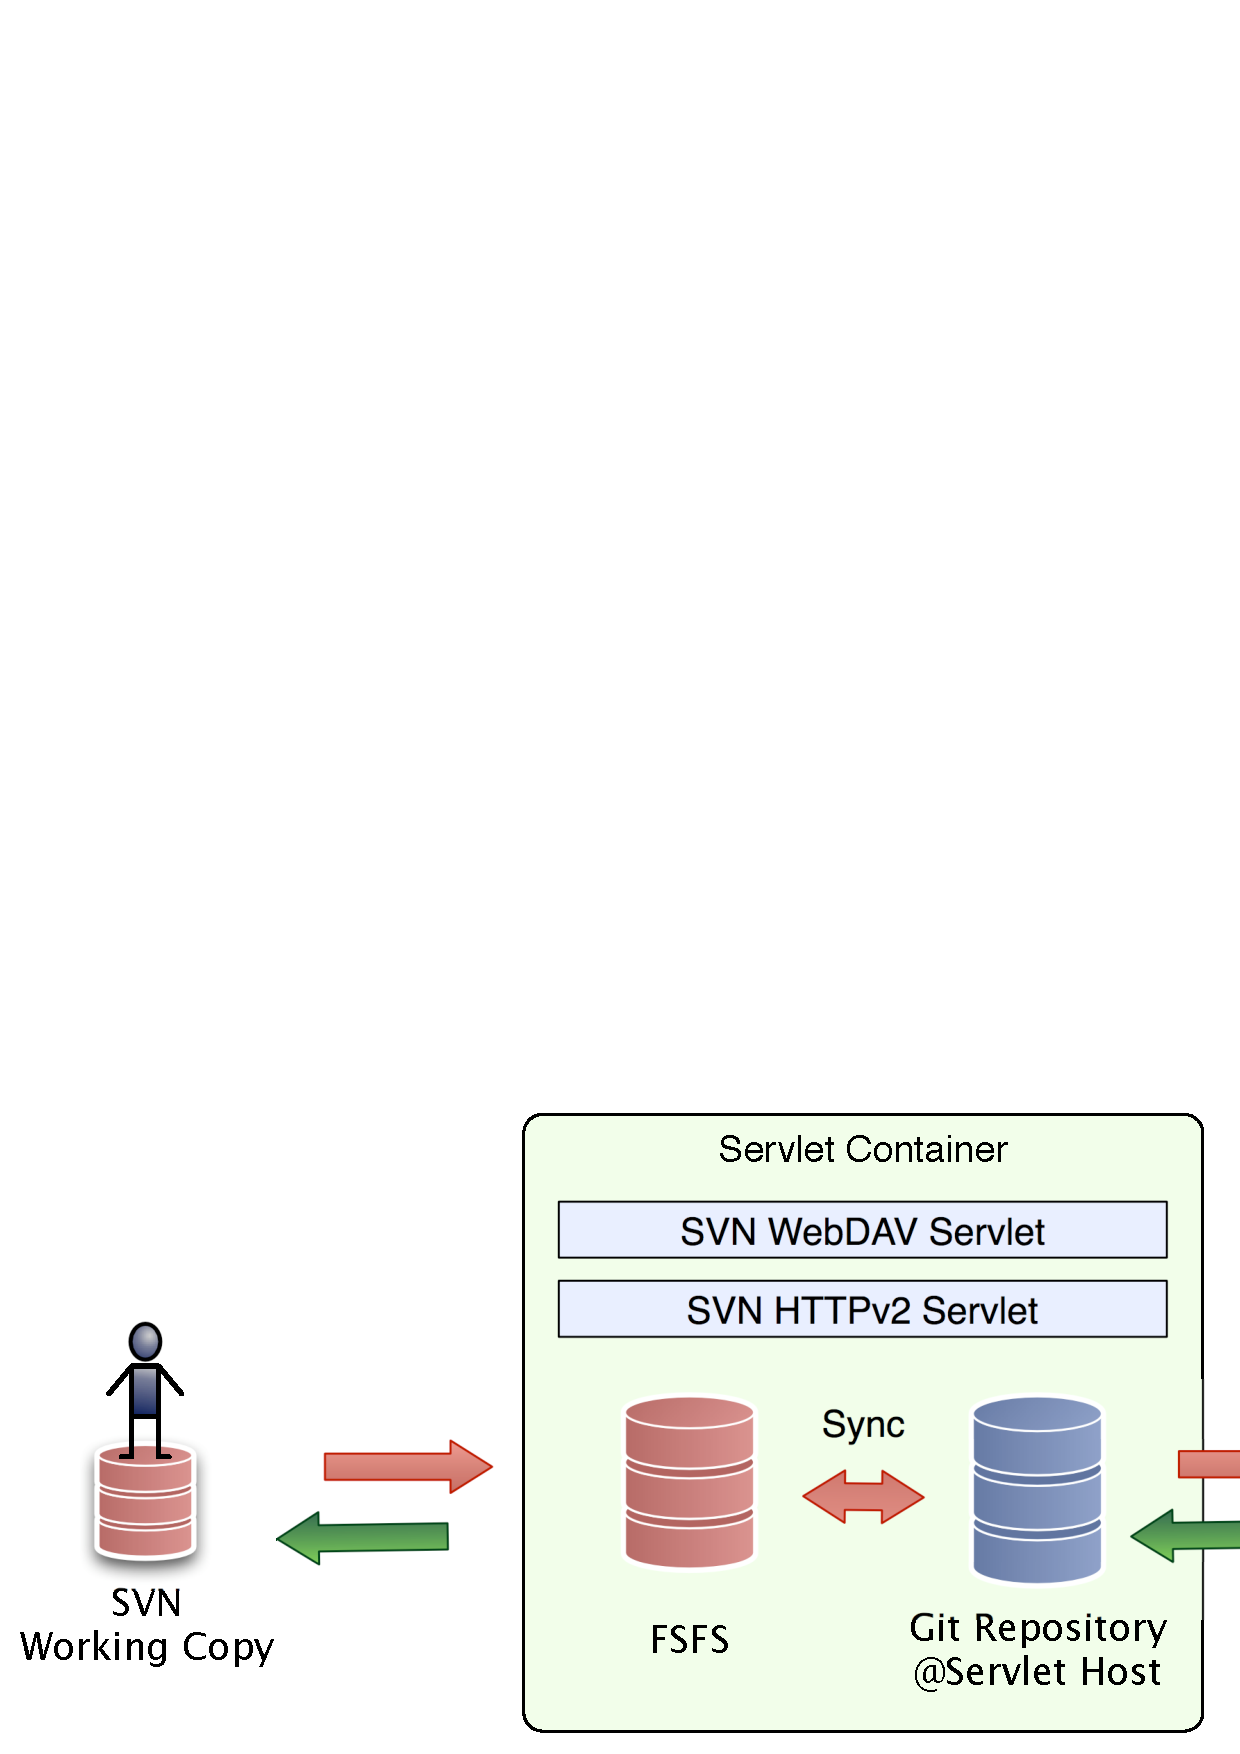
\includegraphics[width=\textwidth]{img/servlet/components_keep_github_safe.pdf}%
\captionof{figure}{Translator Components.}
\label{translator_components_pic}%
\end{center}

Translator major features from the architecture perspective are \emph{maximum level of reuse} of the standard existing components, and \emph{minimum interference} with the existing GitHub infrastructure. 
Let's take a look at how these features are implemented. This chapter provides an overview of Translator components and further chapters provides more details on how each particular operation is carried on.

\label{srp}
\subsubsection{Subversion Requests Processor}
In order to process Subversion user's requests sent over HTTP protocol, Translator is implemented as a Java servlet which might be ran inside any servlet container. All Subversion requests are served by the standard Subversion processing code which serves 
these request by reading from or writing to the local Subversion repository (see FSFS at figure \ref{translator_components_pic}).
\\\\
Processing some of the write requests includes calls to \emph{hooks} which instantly translates Subversion revisions to Git commits.
\\\\
\textbf{Reused:} existing Subversion codebase; Subversion repository as a data storage.\\
\textbf{Interference with GitHub infrastructure:} none. 

\subsubsection{Git to Subversion Translator}
To make any sense, local Subversion repository must be kept up to date with its GitHub counterpart, i.e. it have to include all the changes committed into GitHub repository by Git users. Synchronization of the local Subversion repository with GitHub Git repository is performed in two steps:
\begin{enumerate}
\compactlist
\item Changes in GitHub Git repository are pulled to the local Git repository
\item Git commits from local Git repository are imported into the local Subversion repository
\end{enumerate} 
Synchronization takes place:
\begin{itemize}
\item Before Subversion repository becomes available to the users, to import existing Git commits into Subversion repository
\item Just before Subversion commit is translated into Git commit to make sure Subversion repository is up to date
\item On schedule, to minimize delays on commit
\end{itemize} 
Import of Git commits into Subversion repository is performed with the help of SVNGitKit Java library.
\\\\
\textbf{Reused:} SVNGitKit library to import commits; Git code to clone and fetch from GitHub Git repository into the local one.\\
\textbf{Interference with GitHub infrastructure:} similar to other GitHub clients, this component of Translator clones and then fetches new changes into its clone of GitHub repository.

\subsubsection{Subversion to Git Translator}
Commits made by Subversion users are instantly translated into Git commits which are then pushed into GitHub Git repository. Component responsible 
for that instant translation and push is implemented as \emph{hooks} called by Subversion code during commit (see \ref{srp}).
\newpage 
This approach helps to make sure that Subversion commit and corresponding Git push operation are part of the same transaction and either succeeds or fails together.
For more detailed description of how Subversion commits are processed, refer to the section 1.2 of this specification.
\\\\
\textbf{Reused:} Instant translation uses SVNGitKit library, small part of the code is custom, in particular part which is responsible for integrity of Subversion commit and Git push pair.\\
\textbf{Interference with GitHub infrastructure:} similar to other GitHub clients, this component of Translator performs push of the new Git objects into GitHub Git repository.

\subsubsection{GitHub Integration}

Translator architecture minimizes interference with the existing GitHub infrastructure which is clearly an advantage, but there is a performance penalty being paid for that.
In particular, there is synchronization of the local Git repository with the GitHub Git repository using fetch and push operations. Moreover, both fetch and push are 
performed as part of Subversion commit operation, which might make Subversion commits slow and prone to timeout related errors.
\\\\
To resolve this potential performance issue, Translator could benefit from having local filesystem access to the GitHub repository. Then Translator may work directly with GitHub repository,
with no need to use expensive push and fetch operations.
\begin{center}
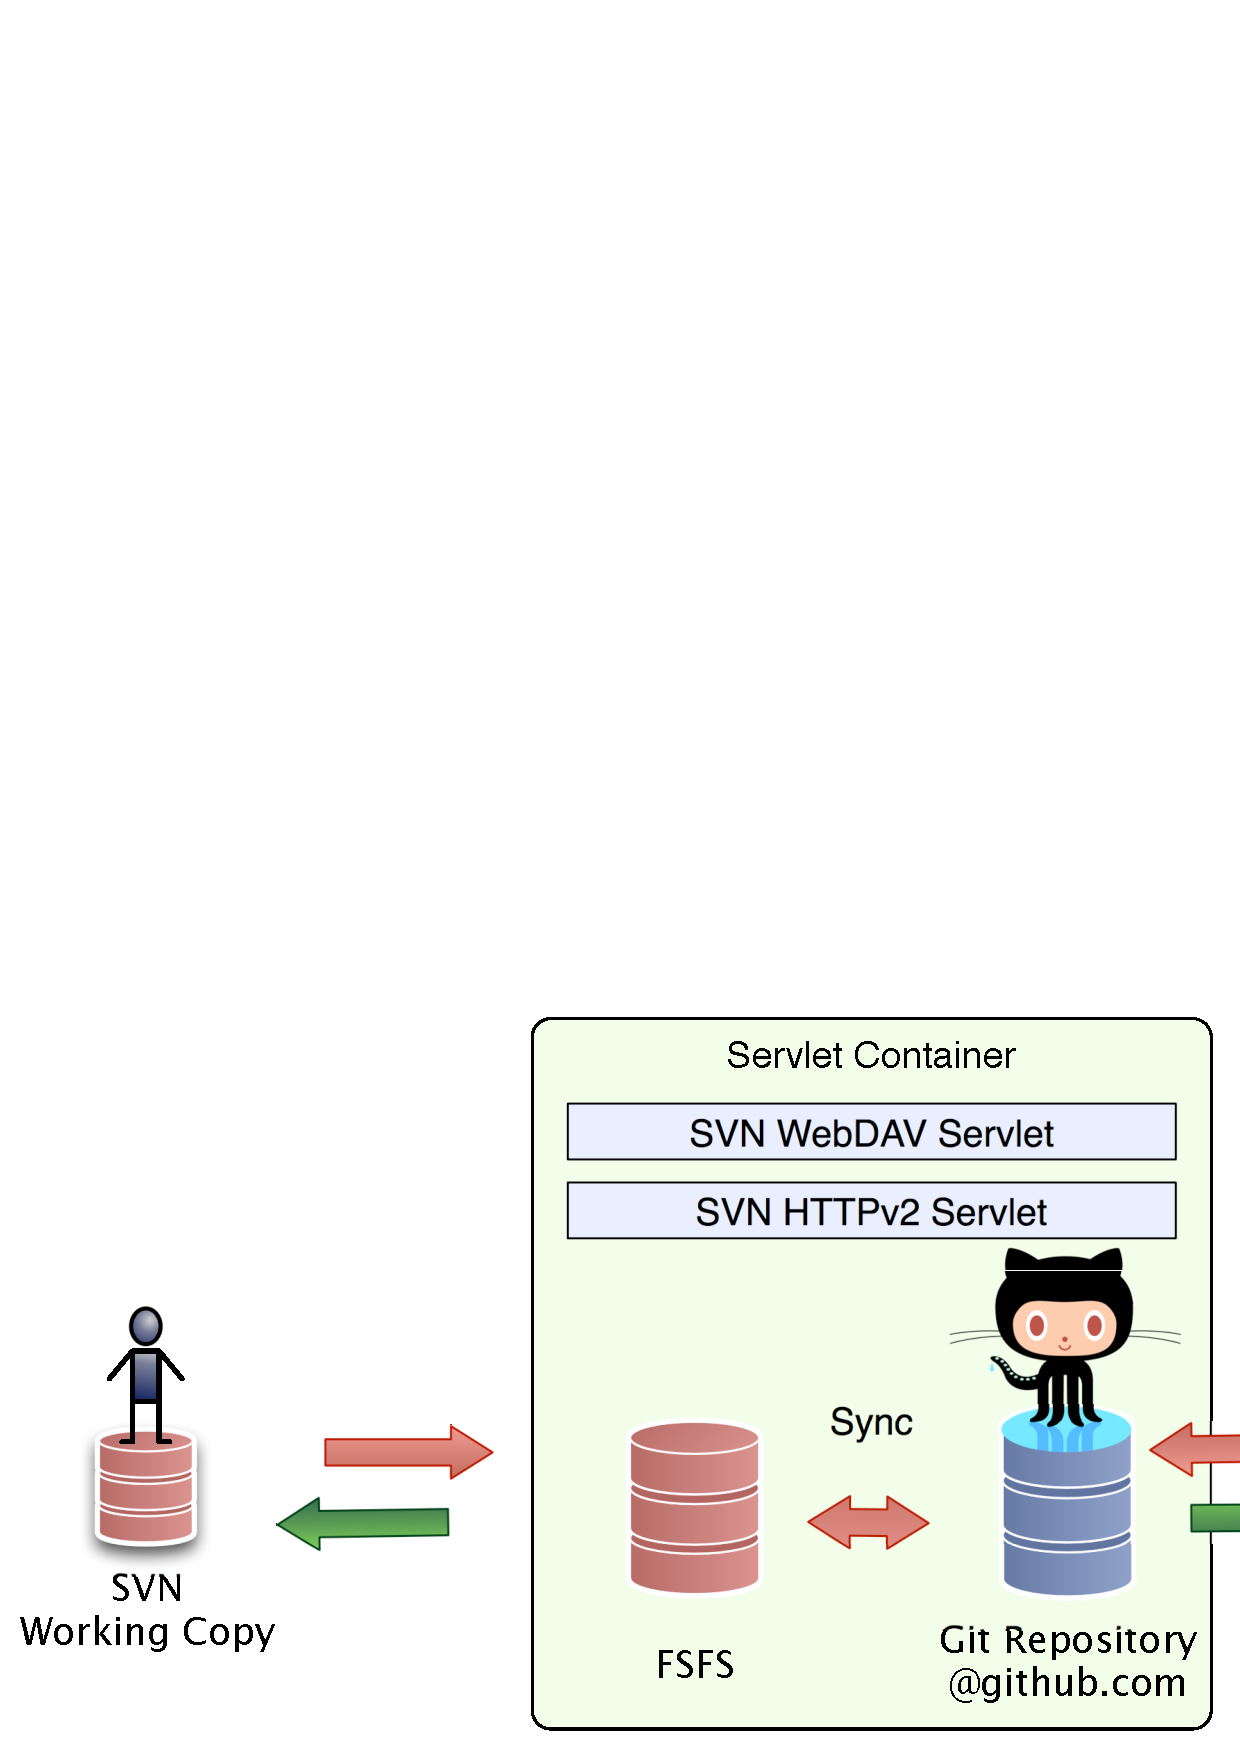
\includegraphics[width=\textwidth]{img/servlet/components_not_that_safe.pdf}%
\captionof{figure}{Higher level of interference.}
\label{translator_components_pic2}%
\end{center}

Major drawback of that solution is that theoretically, bug in Translator code may damage existing GitHub repository contents.
\subsection{Commits to Revisions Mapping}

Translator performs translation of Git commits created by Git users into Subversion revisions, as well
as mirror translation of Subversion revisions created by Subversion users into Git commits. This section
describes how one concept (revision or commit) is mapped into another by Translator and how this mapping 
is stored.

\subsubsection{Git Commits to Subversion Revisions}

Every Git commit is translated to a single Subversion revision which modifies (or creates) a single branch or tag
in Subversion repository. Some of the non-commit changes, like Git branch or tag object creation are also translated into Subversion revisions.\\\\
\begin{figure}[!h]
\label{simple_git_to_svn}
\centering
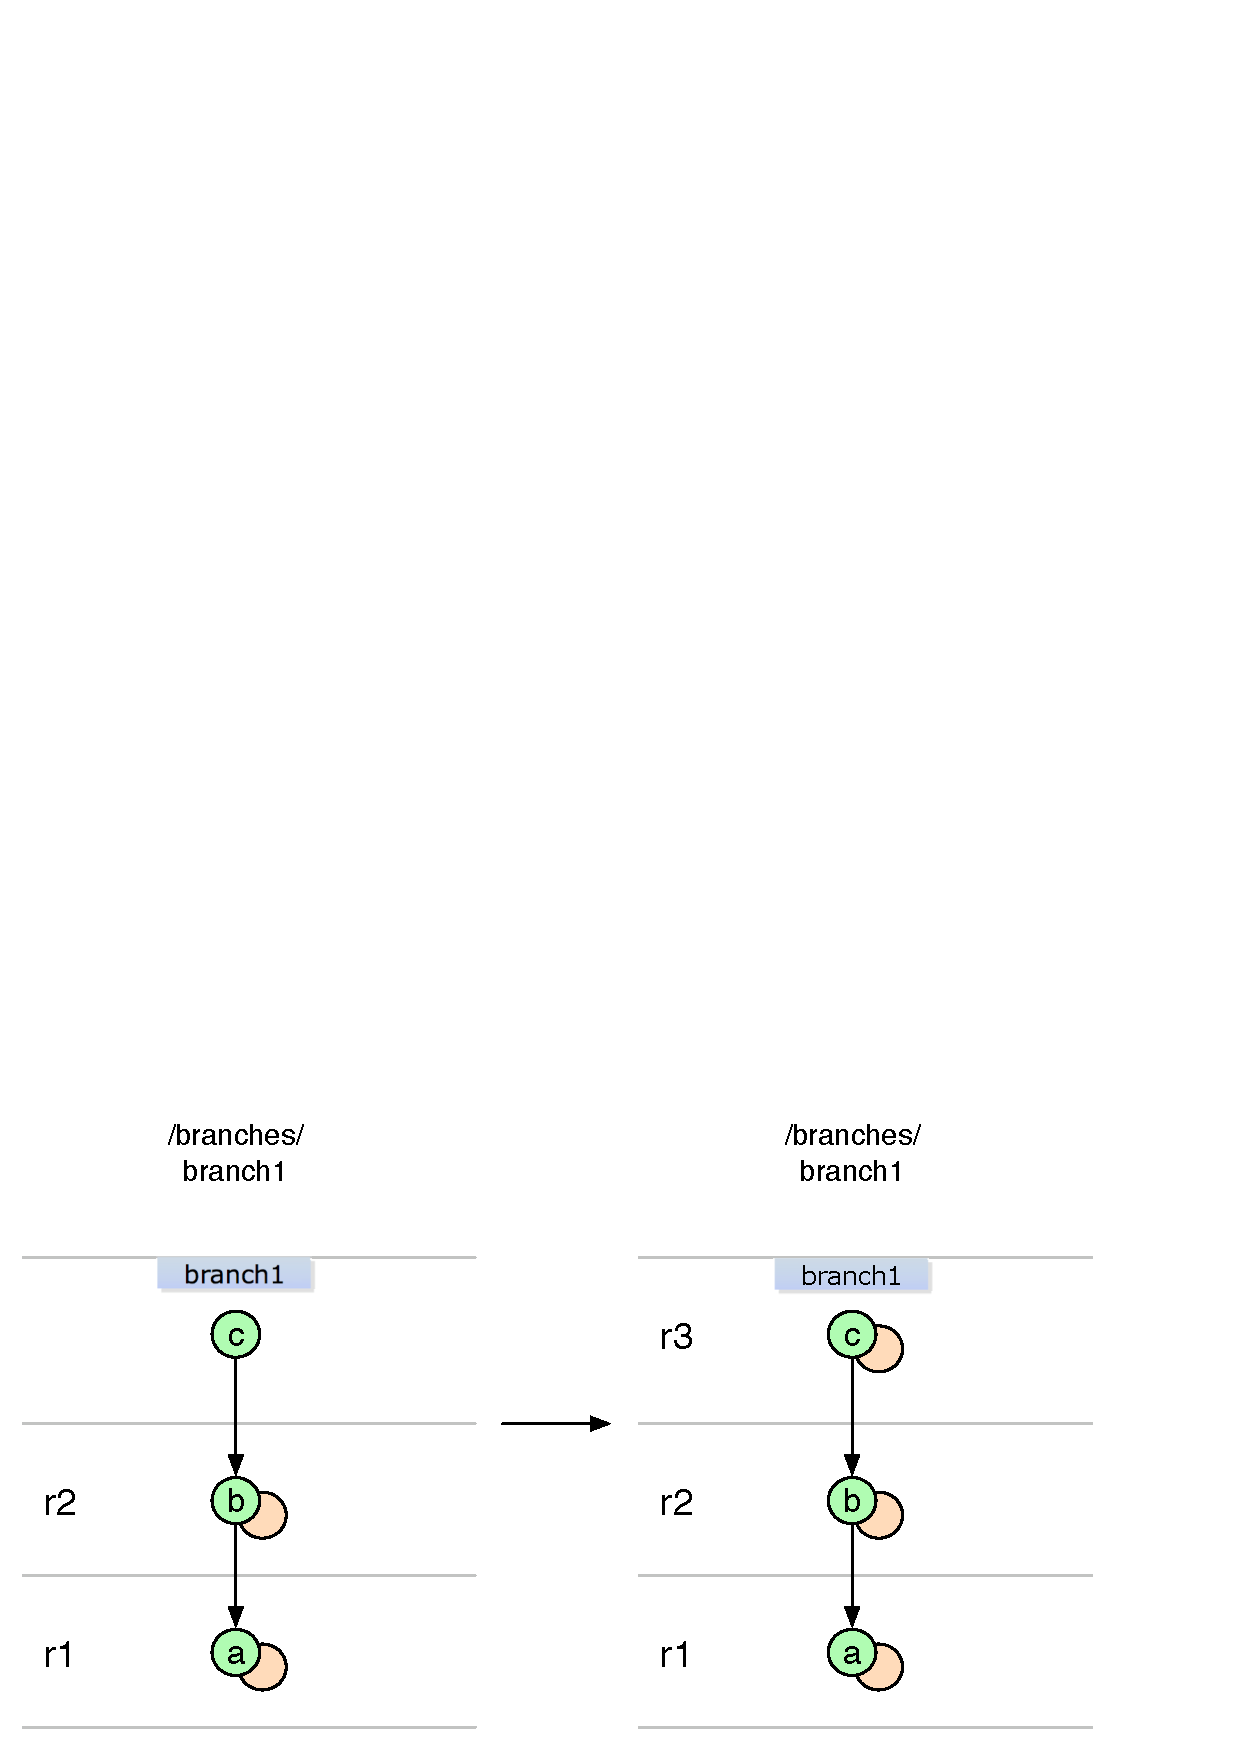
\includegraphics[width=\linewidth]{img/diagrams/single_change_git_to_svn.pdf}
\caption{Git Commit being translated to Subversion Revision}
\end{figure}Mapping between Git commit objects and corresponding revisions in Subversion repository (pair of revision number and branch name) is 
kept in Git repository, in a way similar to the one used to store Git notes. 
\\\\
Translator creates a special branch named /refs/mapping/svn and creates files in this branch named with Git commit object Id - this is the first part of the mapping. 
Contents of the file is Subversion revision number and branch name - second part of the mapping.
\\\\ 
By merging contents /.git/refs/mapping/svn branch to /.git/refs/notes we will get user friendly output of the mapping as part of the standard git log.

\subsubsection{Subversion Revisions to Git Commits}

Every Subversion revision is translated into one or more Git commits, depending on the amount of the branches affected by that particular Subversion commit.\\\\
Mapping between Subversion revision and corresponding Git commits is kept in Subversion repository in form of a special revision property.
\begin{figure}[!h]
\label{simple_svn_to_git}
\centering
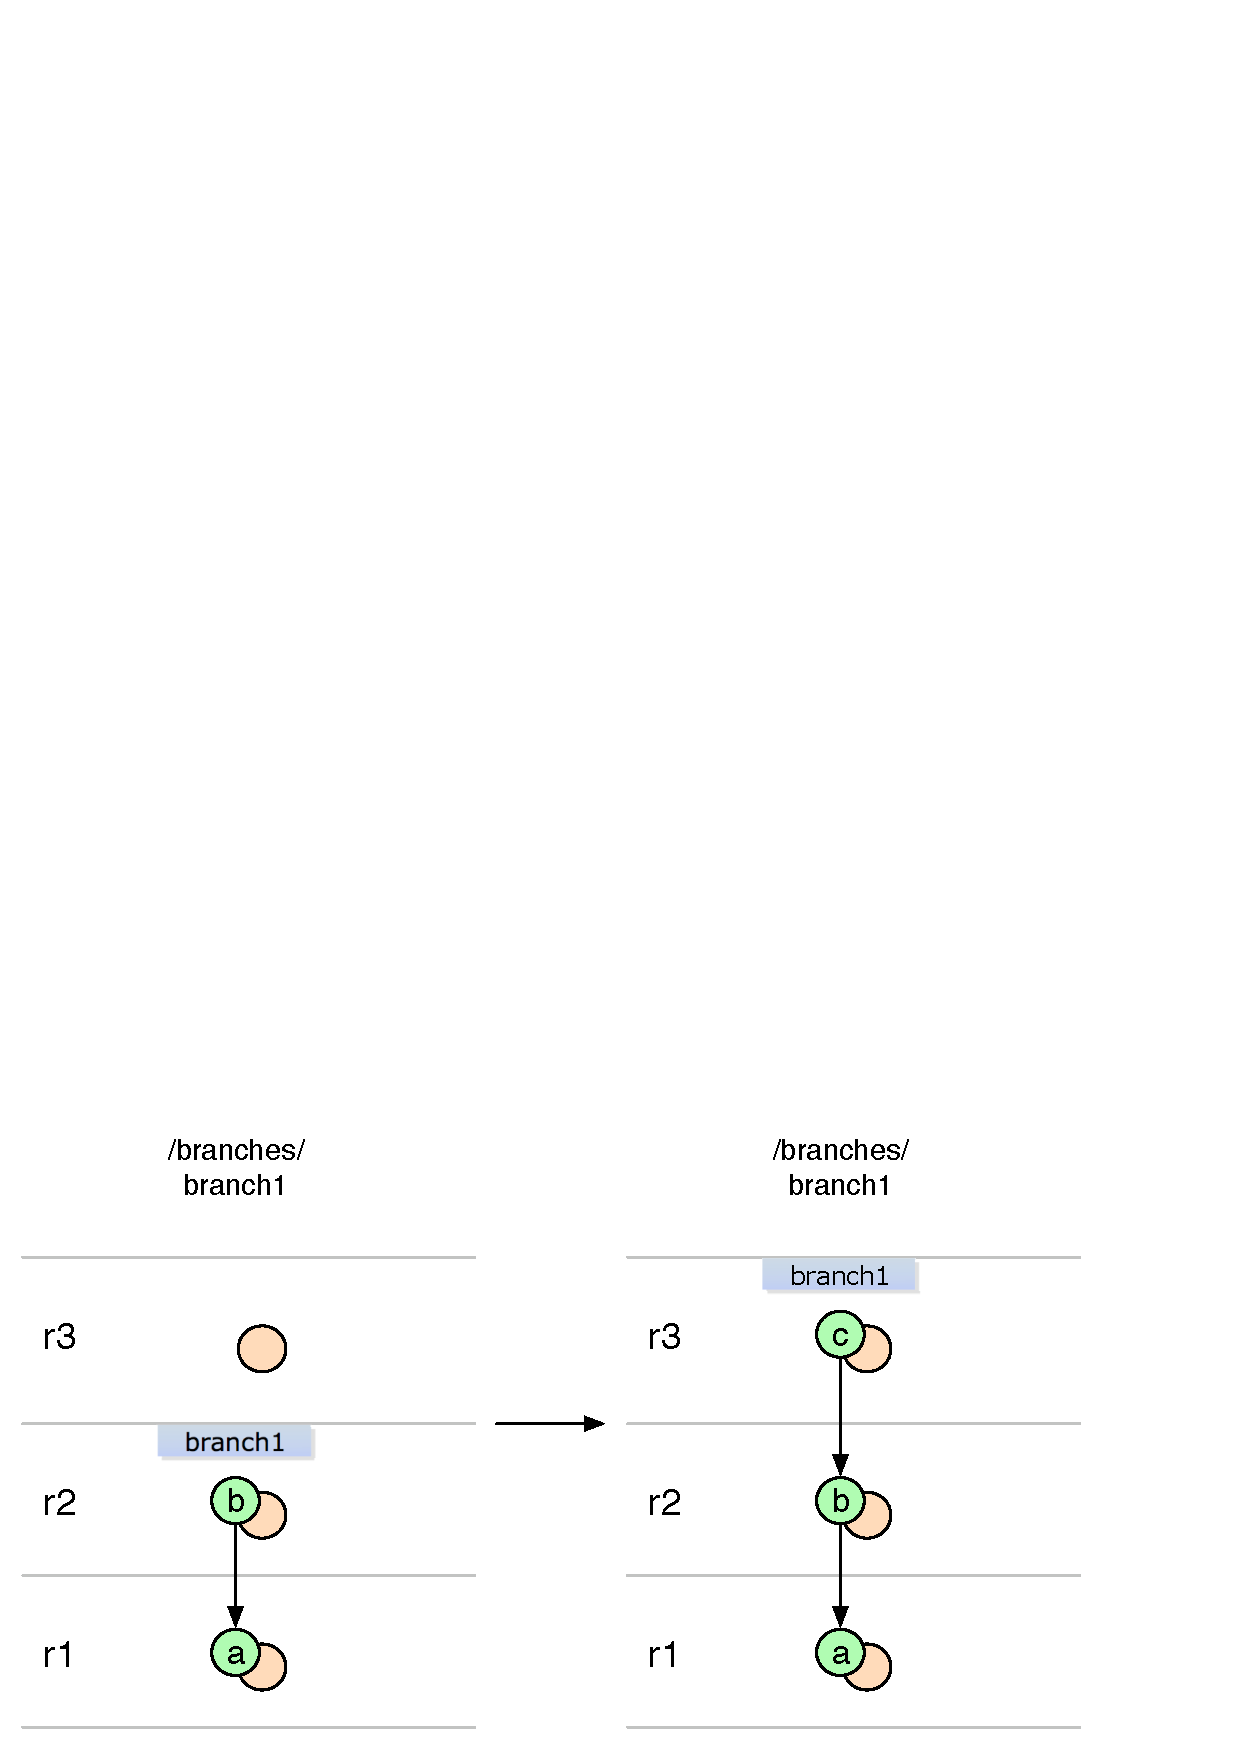
\includegraphics[width=\linewidth]{img/diagrams/single_change_svn_to_git.pdf}
\caption{Subversion Revision being translated to Git Commit}
\end{figure}
\\\\
Both mappings are kept in corresponding repositories (in a special branch and as revision properties), so that no special storage is needed.
\subsection{Processing Subversion Commits}

Translator plugs into the standard Subversion commit process so, that after Subversion commit operation
is completed and new revision is visible to Subversion user, Translator guarantees that translated Git commits
corresponding to this very revision are available to GitHub Git repository users.
\\\\
Thus, Translator guarantess atomicity and integrity of the transaction composed of Subversion commit operation
and Git commit creation and push.
\\\\
Subversion handles user's commit request in the following way:

\begin{enumerate}
\item Commit transaction is constructed from user's description of it. Multiple transactions might be constructed simultaneously.
\item \textbf{Hook 1}
\item \textbf{Hook 2} Commit transaction is then "merged" with the latest repository revision. In case there is a conflict (file modified by transaction might be modified by another transaction already), then out-of-date error is reported and commit is aborted. Otherwise transaction is assigned a base revision.
\item Repository is locked for writing (using file system lock) and in scope of this lock, transaction is converted to the immutable repository revision. In case transaction base revision differs from the actual latest repository revision (which is verified very early), then repository is unlocked and another attempt to merge transaction and reassign base revision to it is performed (go to 2).
\item \textbf{Hook 3} Repository latest revision (visible to the users) is updated atomically and repository is unlocked.
\end{enumerate}
To perform instant translation and push, Translator plugs into \textbf{Hook 1}, \textbf{Hook 2} and \textbf{Hook 3} points of the commit handling process.
\\\\
\textbf{Hook 1:} Local Git repository synchronized with its GitHub origin. Local Subversion repository is synchronized with the local Git repository.
\\\\
\textbf{Hook 2:} Git Commit objects are created, Git braches and tags modified accordingly to the translation rules.
\\\\
\textbf{Hook 3:} Local Git repository changes are pushed to GitHub origin repository.
\\\\
This way, unless Subversion commit succeeded, no Git translation and push will take place and unless push have succeeded, new Subversion revision will not become visible.

\subsection{Processing Git Commits}

No special actions are taken on Git commits. This helps to make sure that Git workflow is not interrupted and not slowed down by
the mere presence of the Translator.
\\\\
All necessary translation of Git repository to Subversion one might be performed on demand, at the time there is real user's request
to Subversion server, or in advance in case user have scheduled such translation or agreed on some overhead connected to Translator
working with user's repository.
\subsection{Fixed Subversion Repository Layout}

To support sane translation of Git branches and tags concepts into correspoding Subversion concepts, Translator must enforce certain Subversion repository layout and introduce limitations which are not present in the standard Subversion repository. 
In practice, these limitations will have no or very limited influence on real Subversion use cases.
\\\\
\textbf{Layout:}\\ 
Subversion repository always has the following directories:
\\\\
/trunk\\
/branches\\
/tags\\\\
\textbf{Limitations:}
\begin{enumerate}
\item no directories or files may be created in the root of repository
\item /trunk, /branches and /tags directories may not be deleted or copied
\item /branches/\emph{B} directory may only be created as a copy of /trunk or
as a copy of another /branches/\emph{A} directory
\item /tags/\emph{T} directory may only be created as a copy of /trunk or
as a copy of another /tags/\emph{A} or /branches/\emph{B} directory
\item no directory except of direct children of /tags or /branches might be a
copy of /trunk or of /tags/\emph{T} or of /branches/\emph{B} directory
\item no files might be created in /tags and in /branches directories
\end{enumerate}
Above layout and listed limitations corresponds exactly to the Subversion common practice informal standard which
is used in case when Subversion repository contains a single project. Subversion does not encourage people 
to keep multiple projects in the same repository, but some users may prefer the following layout:
\\\\
/projectX/trunk\\
/projectX/branches\\
/projectX/tags\\
/projectZ/trunk\\
/projectZ/branches\\
/projectZ/tags\\\\
or any other combination of the standard layout components and project or subsystem names. Translator does not support such layouts as they 
makes sane branches and tags concepts translation more complicated and ambigous.


\newpage
\hrule
\section{Translated Concepts}
\subsection{Revisions and Commits}

Both revision in subversion and commit in git are atomic changes fixed at certain moment in time by certain person with certain message. This metadata of change is always translated as follows:
\begin{enumerate}
\compactlist
\item Time
\item Author
\item Commit message
\end{enumerate}
\subsection{Branches and Tags}

Technically Subversion does not introduce separate concepts for branches and tags. Both branches and tags are versioned directories under repository root. As result Translator performs theirs translation in similar way. There are differences at Git level only:
\begin{enumerate}
	\compactlist
	\item Addition.
	\begin{itemize}
		\item Creation of /branches/\emph{B} directory leads to creation of a new branch reference \emph{B}.
		\item Creation of /tags/\emph{T} directory leads to addition of corresponding Tag Object with name \emph{T}.
	\end{itemize}
	\item Modification.
	\begin{itemize}
		\item Change at /branches/\emph{B} directory leads to updating of corresponding branch reference \emph{B}.
		\item Change at /tags/\emph{T} directory leads to the removal of obsolete Tag Object with name \emph{T} and creation of new Tag Object with the same name for corresponding Commit Object.
	\end{itemize}
	\item Deletion.
	\begin{itemize}
		\item Removal of /branches/\emph{B} directory leads to removal of corresponding reference \emph{B} at Git repository, when
		\item Removal of /tags/\emph{T} directory leads to removal of corresponding Tag Object with name \emph{T}.
	\end{itemize}
\end{enumerate}

The same rules could be treated in opposite direction --- every change of Git branch or tag leads to corresponding change of Subversion branch or tag.

This and further chapters consider scenarios with branches only. But every scenario could be applied to tags with the rules above taken into account.

\subsubsection{From Subversion to Git}

There is a number of ways to create branch in Subversion.

\begin{enumerate}
\compactlist
\item Branch creation by copying, figure \ref{branch_creation_svn_to_git}.

\begin{figure}[!h]
\centering
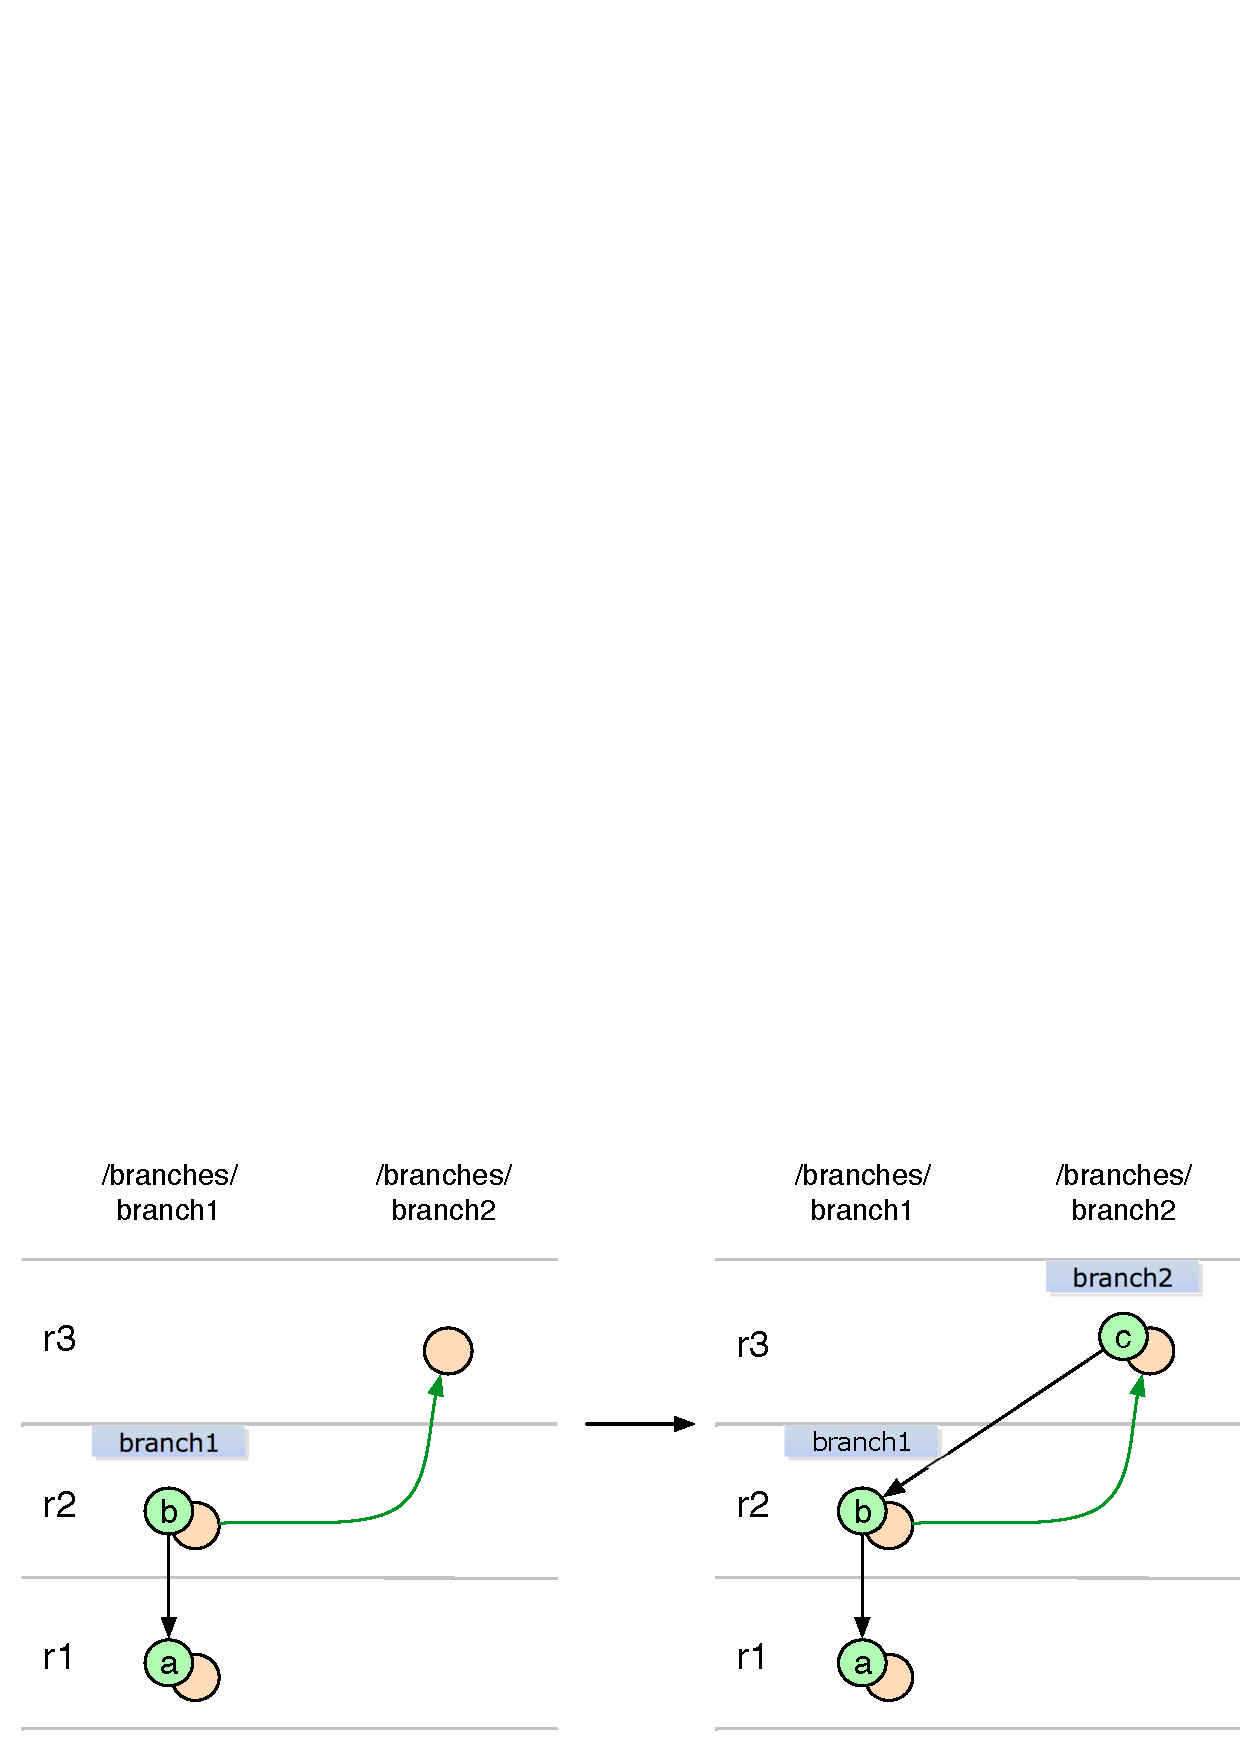
\includegraphics[width=\linewidth]{img/diagrams/branch_creation_svn_to_git.pdf}
\caption{Subversion branch copying being translated to Git branch creation.}
\label{branch_creation_svn_to_git}
\end{figure}

% end of item
\item Branch addition with merge history. See \ref{branch_creation_from_mergeinfo_svn_to_git}.

\begin{figure}[!h]
\centering
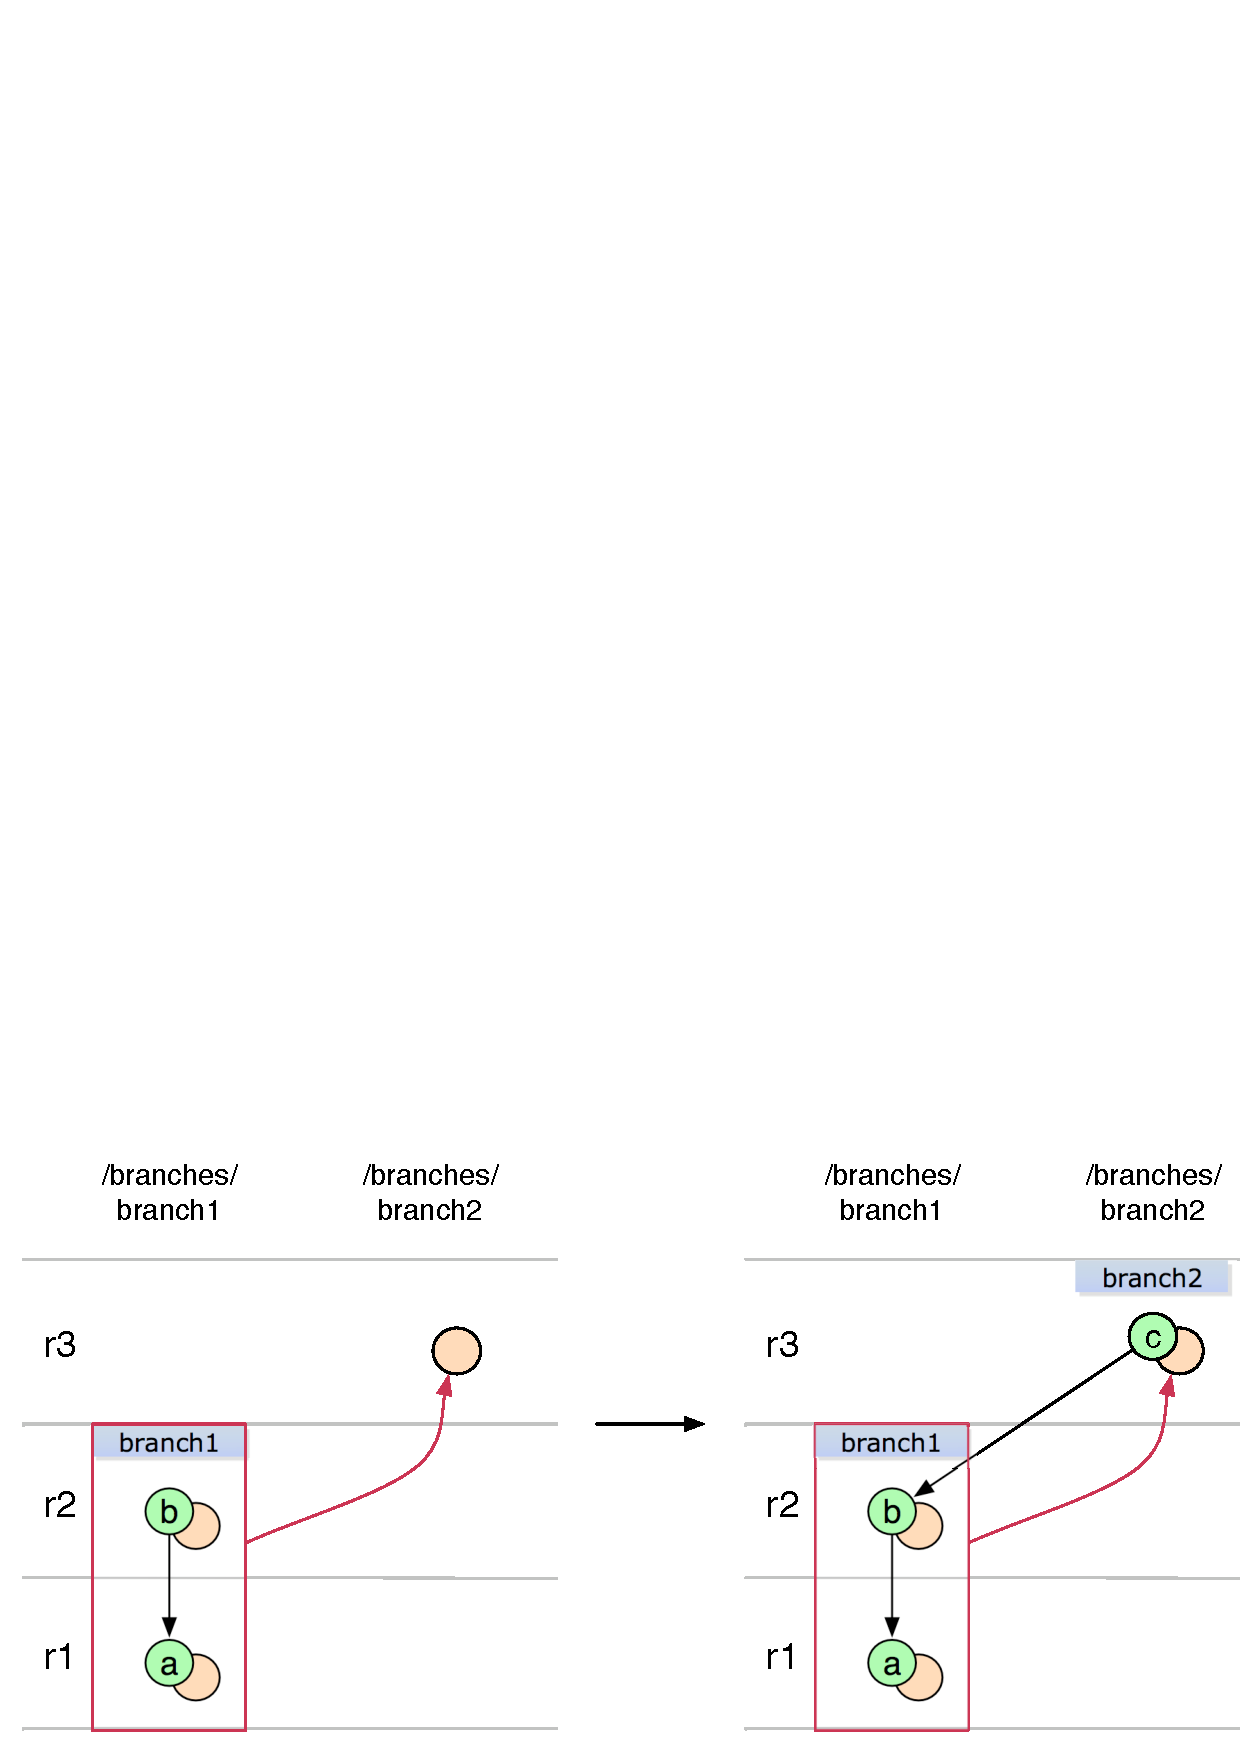
\includegraphics[width=\linewidth]{img/diagrams/branch_creation_from_mergeinfo_svn_to_git.pdf}
\caption{Subversion branch addition being translated to Git branch creation.}
\label{branch_creation_from_mergeinfo_svn_to_git}
\end{figure}

\item Branch addition with no history.

This kind of translation basically consists of:
\begin{enumerate}
	\item Creation of new commit object with no parents attached to it.
	\item Adding a branch reference to this new commit afterwards.
\end{enumerate}

\end{enumerate}

\subsubsection{From Git to Subversion}

\begin{enumerate}
\compactlist
\item Branch creation and committing on new branch, figure \ref{branch_creation_git_to_svn}.

\begin{figure}[!h]
\centering
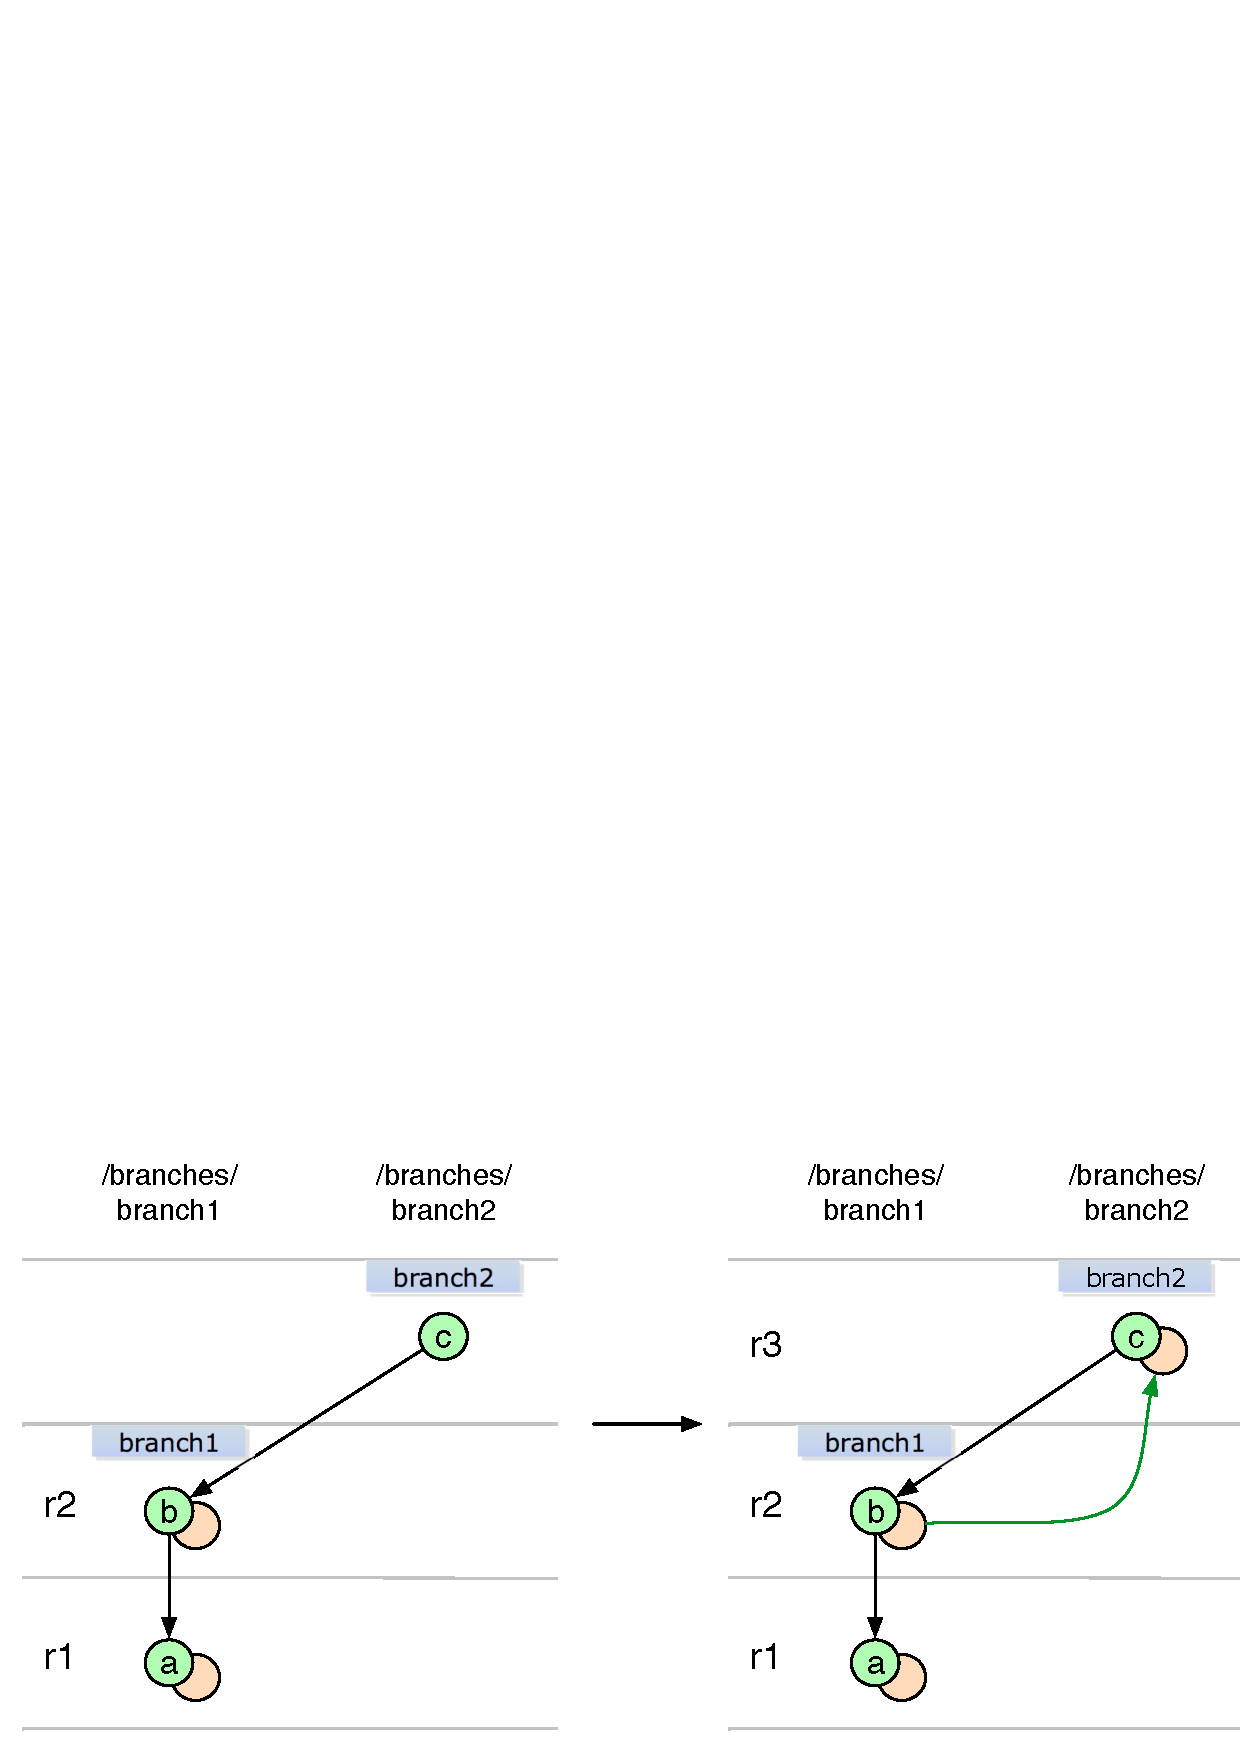
\includegraphics[width=\linewidth]{img/diagrams/branch_creation_git_to_svn.pdf}
\caption{Commit on Git branch being translated to Subversion.}
\label{branch_creation_git_to_svn}
\end{figure}

\item Branch reference creation with no commit, figure \ref{svn_no_change_branch_creation_git_to_svn}.

\begin{figure}[!h]
\centering
\includegraphics[width=\linewidth]{img/diagrams/svn_no_change_branch_creation_git_to_svn.pdf}
\caption{Commit on Git branch being translated to Subversion.}
\label{svn_no_change_branch_creation_git_to_svn}
\end{figure}

\item Double branch reference creation and committing on new branches, figure \ref{ambiguous_svn_branch_git_to_svn}.

\begin{figure}[!h]
\centering
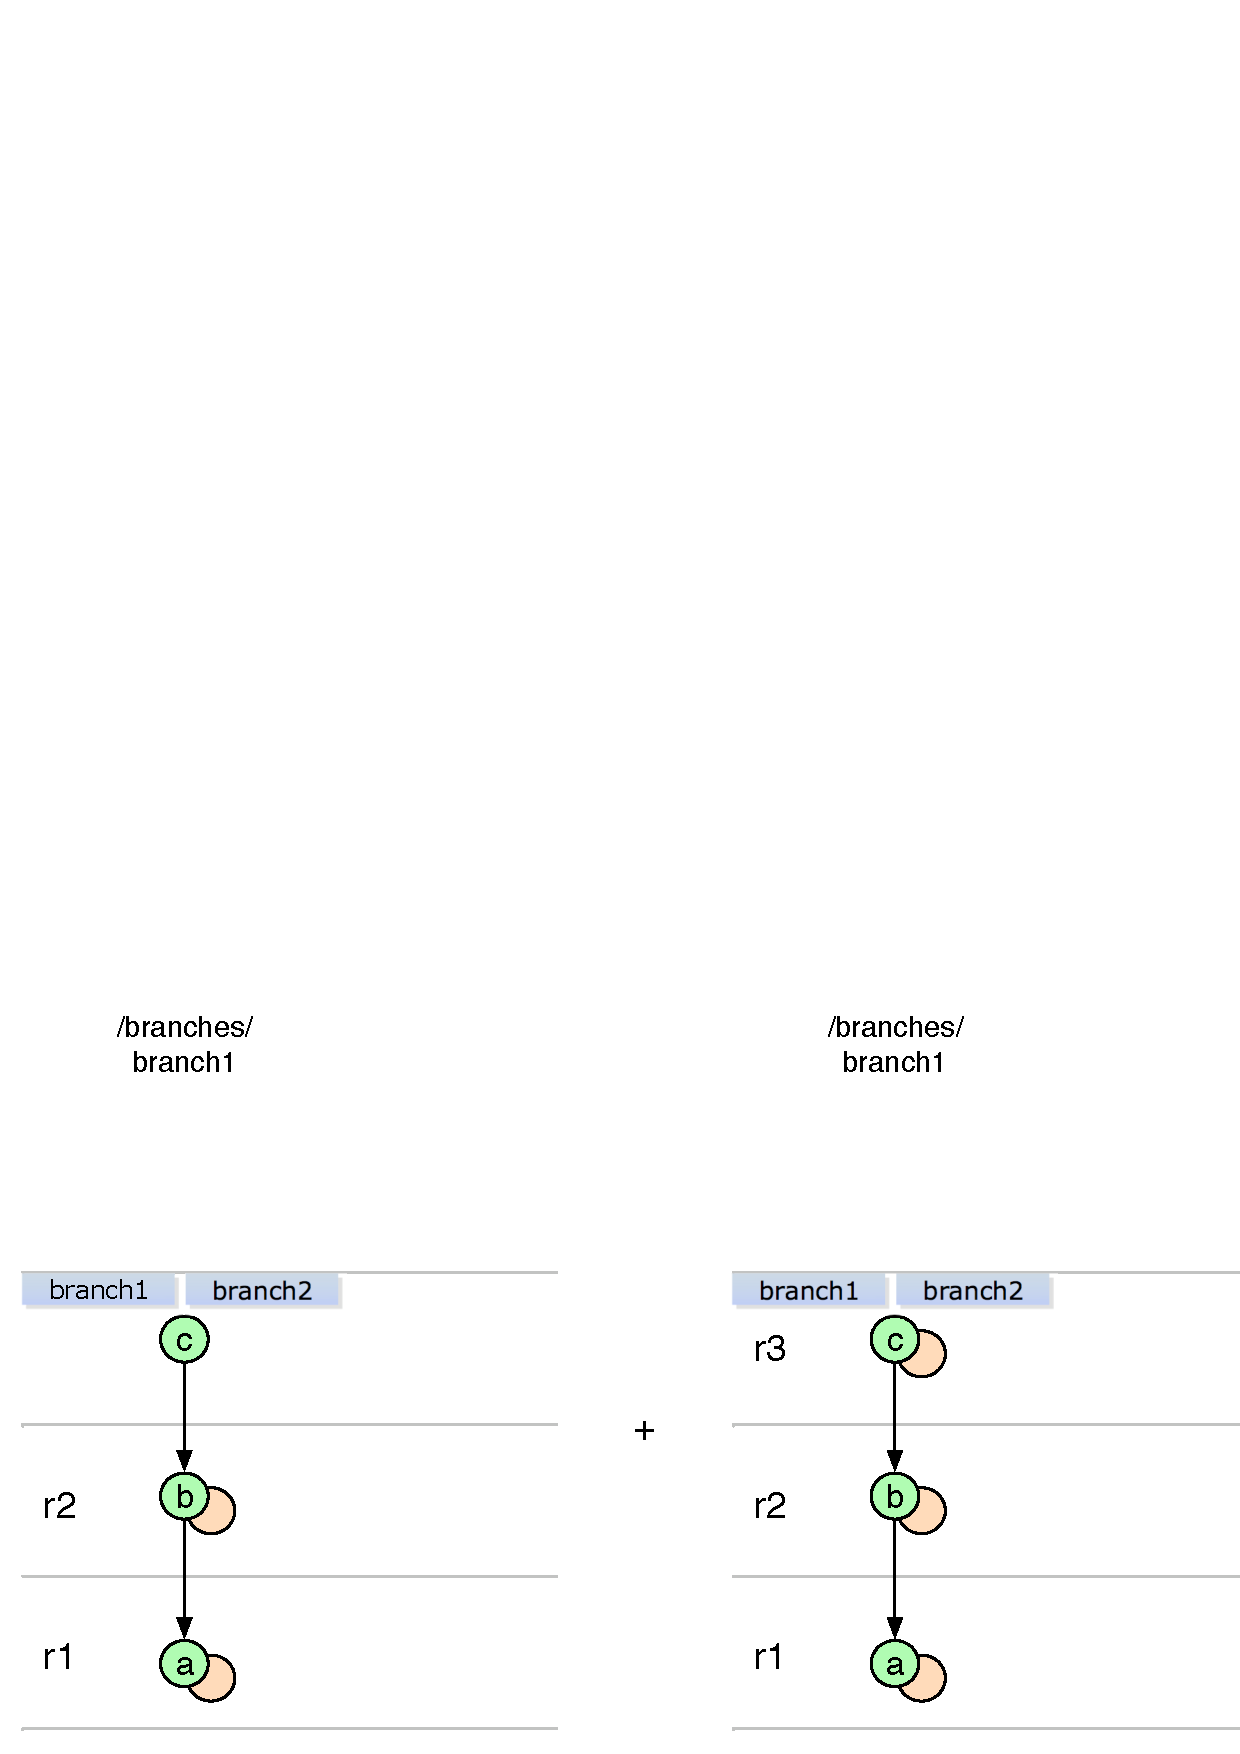
\includegraphics[width=\linewidth]{img/diagrams/ambiguous_svn_branch_git_to_svn.pdf}
\caption{Commit on Git branch being translated to Subversion.}
\label{ambiguous_svn_branch_git_to_svn}
\end{figure}

\end{enumerate}

\subsection{Merge}
\renewcommand{\figurename}{Diagram}
\subsection{Copies and Renames}
This section describes translation of files and directories copies and renames, \emph{other than} copies and renames of 
branches (/branches/\emph{B}) and tags (/tags/\emph{T}). For that sort of copies and renames refer to the "Branches and Tags" 
section of this specification.\\\\
Rename translation does not differ from translation of the copy, because both Git and Subversion
express renames as a composition of copy and deletion.% I'd say it's a huge gap between copy detection and rename detection in Git, since it's a heavy task for Git to find copies, when it works just fine with rename detection. From this point I suggest (and SVNGitKit currently behaves this way) that we detect renames only at Git to SVN translation, at least for the first release.

\subsubsection{Copies in Subversion to Git}
No special translation is performed for a file or directory copied or renamed in Subversion revision. Copy of the single file is translated 
to creation of a new file in the corresponding Git commit. Copy of a directory is translated to creation of a new directory with all its children
in the corresponding Git commit.

\subsubsection{Copies in Git to Subversion}
Whenever it is revealed that new file in Git commit is a result of copy or rename, this new file creation is translated to a file copy in the 
corresponding Subversion revision.\\\\ 
When amount of copied files in a new directory exceeds certain threshold (percentage of the amount of files in the original directory), then new directory
creation is translated into a directory copy with appropriate directory content adjustment in the corresponding Subversion revision.
\subsection{Properties and Attributes}
This section describes translation rules for the metadata set on repository files and directories in Git or Subversion.
Aim of Translator is to preserve meaning of the metadata information while translating from one version control 
to another.
\\\\
Subversion keeps metadata in form of versioned properties that could be set on any file or directory in the repository.
Properties might have any name, but there are number of reserved names, with \emph{svn:} prefix for special properties. 
These special properties, been set on a file or directory, controls various aspects of Subversion client behaviour, 
from EOL substitution to support of the external repositories.
\\\\
Git has multiple ways to keep metatada, these ways are:
\begin{enumerate}
\compactlist
\item Every directory and file has \emph{file mode} bytes stored at repository;
\item \emph{.gitignore} file stores file path patterns to be ignored by Git operations;
\item \emph{.gitattributes} is a file in a special format that could be present in any directory.
This file allows to define special metadata attributes per file.
\end{enumerate}

Translation rules for the metadata properties and attributes are described in further sections.

\subsubsection{End-of-Line Bytes and MIME Types}
Subversion supports EOL bytes substitution since its early versions. 
Support of different EOL-styles was introduced in Git at version 1.7.2. Taking this in account, 
Translator will perform valid EOL translation only for the users of Git version 1.7.2 or newer.
\\\\
EOL substitution only makes sense for text files only. Thus, in this specification, rules 
for translating EOL-style and MIME-type metadata are combined. 
\\\\
\textbf{Subversion to Git Translation}
\\\\
Subversion uses svn:eol-style and svn:mime-type properties set on individual files to keep corresponding kinds of metadata.
Value of these properties set on a file are translated into the corresponding lines in \emph{.gitattributes} file, which ensures that 
corresponding file in the Git repository has proper \emph{eol} and \emph{text} attributes set.
\\\\
Upon translation of these properties Translator tries to minimize amount of modifications
made to .gitattributes files. To translate svn:eol-style and svn:mime-type properties changes, 
Translator uses the following algorithm:

\begin{enumerate}
\compactlist
\item For every file wich has svn:eol-style or svn:mime-type property modified, Translator looks for a corresponding line in one of .gitattributes files located in the parent directory or 
at the higher level of the directories hierarchy.\\
	
\item If attribute line is found, Translator adjusts corresponding attribute to reflect performed change. Basically Translator adds a line with pattern corresponding to the path of modified file and a new attribute:\\\\
\emph{/$<$relative-file-path$>$ $<$text-related-value$>$ $<$eol-related-value$>$},\\\\
where $<$text-related-value$>$ and $<$eol-related-value$>$ are generated according to the rules defined in the table \ref{eol_mime_svn_to_git}.\\
	
\item If no .gitattributes file was found in the ancestor directories of the file, Translator creates new .gitattributes file in the parent directory of the file with the following contents:\\\\
\emph{/$<$file-name$>$ $<$text-related-value$>$ $<$eol-related-value$>$},\\\\
where $<$text-related-value$>$ and $<$eol-related-value$>$ are generated according to the rules specified at table \ref{eol_mime_svn_to_git}.\\
	
\item If more than one .gitattributes file was found in the parent directories of the file, then the closest one is chosen. 
Translator appends the following line to the selected .gitattributes file:\\\\
\emph{/$<$relative-file-path$>$ $<$text-related-value$>$ $<$eol-related-value$>$},\\\\
where $<$text-related-value$>$ and $<$eol-related-value$>$ are generated according to the rules specified at table \ref{eol_mime_svn_to_git}.\\
\item Finally, for each created or modified .gitattributes file, Translator compacts added rules transforming 
explicit path patterns to the recursive path patterns when possible.
\end{enumerate}

\emph{Note}: comments stored in .gitattributes file left unmodified by Translator.\\
\emph{Note}: Git user must set \emph{core.eol} configuration parameter to allow correct handling of the \emph{native} value of svn:eol-style property.

\begin{center}
\begin{tabular}{ | p{0.20\textwidth} | p{0.20\textwidth} | p{0.20\textwidth} | p{0.20\textwidth} |}
	\hline
	svn:eol-style &   svn:mime-type &   text  & eol \\ \hline \hline
	-             &   text/-        &   unset & undef \footnotemark[1] \footnotemark[2] \\ \hline
	-             &   binary        &   unset & undef \\ \hline
	lf            &   text/-        &   set   & lf \\ \hline
	lf            &   binary        &   unset & undef \\ \hline
	cr            &   text/-        &   unset & undef  \footnotemark[3] \\ \hline
	cr            &   binary        &   unset & undef \\ \hline
	crlf          &   text/-        &   set   & crlf \\ \hline
	crlf          &   binary        &   unset & undef \\ \hline
	native        &   text/-        &   set   & undef \footnotemark[4] \\ \hline
	native        &   binary        &   unset & undef \\ \hline
\end{tabular}
\captionof{table}{Subversion to Git EOL and MIME translation.}
\label{eol_mime_svn_to_git}
\footnotetext[1]{\emph{undef}, in general, needs only to be set, if there is another rule which matches the file, otherwise we may skip these attributes at all.}
\footnotetext[2]{Missing Subversion properties mean text, leave EOLs as is for that case.}
\footnotetext[3]{Subversion recognizes CR EOL-style, Git does not.}
\footnotetext[4]{svn:eol-style property value \emph{native} should stay the same, Git user may configure \emph{native} via \emph{core.eol} configuration property.} 
\end{center}
\newpage
\textbf{Git to Subversion Translation}\\

When .gitattributes file is modified in Git commit, Translator uses the following algorithm steps to apply changes to the metadata of corresponding files in Subversion repository:

\begin{enumerate}
\compactlist
\item For every file affected by the change new svn:eol-style and svn:mime-type properties are computed accordingly to the rules defined in the table \ref{eol_mime_git_to_svn}.
\item When there are no changes detected, Translator performs no further actions.
\item When new and old properties values differ only in those values which were computed from \emph{undef} attribute value, Translator performs no further actions.
\item Otherwise Translator sets new properties to affected files.
\end{enumerate}

\begin{center}
\begin{tabular}{ | p{0.20\textwidth} | p{0.20\textwidth} | p{0.20\textwidth} | p{0.20\textwidth} |}
	\hline
	text  & eol      &  svn:eol-style  &  svn:mime-type \\ \hline \hline
	unset & undef    &  -              &  -/binary \footnotemark[1] \\ \hline
	unset & unset    &  -              &  -/binary \footnotemark[2] \\ \hline
	unset & set      &  native         &  - \footnotemark[3] \\ \hline
	unset & lf       &  lf             &  - \\ \hline
	unset & crlf     &  crlf           &  - \\ \hline
	set   & undef    &  native         &  - \\ \hline
	set   & unset    &  native         &  - \footnotemark[4] \\ \hline
	set   & set      &  native         &  - \\ \hline
	set   & lf       &  lf             &  - \\ \hline
	set   & crlf     &  crlf           &  - \\ \hline
	auto  & undef    &  native/-       &  -/binary \footnotemark[1] \\ \hline
	auto  & unset    &  native/-       &  -/binary \footnotemark[5] \\ \hline
	auto  & set      &  native/-       &  -/binary \\ \hline
	auto  & lf       &  lf/-           &  -/binary \\ \hline
	auto  & crlf     &  crlf/-         &  -/binary \\ \hline
\end{tabular}
\captionof{table}{Git to Subversion EOL and MIME translation.}
\label{eol_mime_git_to_svn}
\footnotetext[1]{Perform binary check.}
\footnotetext[2]{unset/unset is redundant, treat it like unset/undef.}
\footnotetext[3]{From Git documentation:\\eol - This attribute sets a specific line-ending style to be used in the working directory. It enables end-of-line normalization without any content checks, effectively setting the text attribute.}
\footnotetext[4]{set/unset is contradiction, but text has precedence over eol, hence treat like set/undef.}
\footnotetext[5]{auto/unset is contradiction, but text has precedence over eol, hence treat like auto/undef}
\end{center}

\subsubsection{Symbolic Links}
Git stores symbolic link as an entry at Tree Object with a special file mode and corresponding blob containing \emph{path/to/target}.
\\\\
Subversion represents symbolic link as a file with content \emph{link path/to/target} and a property svn:special set on it.
\\\\
So translation is performed by adding or removing \emph{link } prefix to the file content and setting the mode or the property.
\\\\
If file at Subversion repository has svn:special property but its content doesn't start with \emph{link } prefix, it is considered as an ordinary file and translated as a blob.

\subsubsection{Executables}
In Git repository, exectuable files are marked with a special file mode. Executable file in Subversion repository keeps svn:executable property. 
Thus, svn:executable property is translated into Git file mode and vice versa directly.

\subsubsection{Ignores}
Subversion uses svn:ignore property which may be set on a directory to define a list of
file name patterns. Files in this very directory that match at least one of the patterns are ignored.
\\\\
Git uses versioned .gitignore file to define file path patterns to be ignored. Files in the directory
where .gitignores file is located as well as files in the child directories are matched against defined patterns.
\\\\
\textbf{Subversion to Git Translation}
\\\\
Upon translation of the svn:ignore properties changes Translator tries to minimize amount of modifications
made to .gitignore files. To translate svn:ignore properties changes, Translator uses the following algorithm:

\begin{enumerate}
\compactlist
\item For every directory with modified svn:ignore property Translator looks for a corresponding line in one of the 
.gitignore files located in the parent directory or at the higher level of the directories hierarchy.\\
\item If ignore pattern line is found, Translator adjusts corresponding ignore rule to reflect performed change. 
Translator adds a line:\\\\
\emph{/$<$relative-file-path$>$/$<$ignore-pattern$>$}\\
if svn:ignore property was added or modified, and \\\\
\emph{!/$<$relative-file-path$>$/$<$ignore-pattern$>$}\\
if svn:ignore property was removed from the directory.\\
\item If no .gitignore file was found was found in the ancestor directories of the file, Translator creates a new .gitignore file in the file's directory with the following contents:\\\\
\emph{/$<$ignore-pattern$>$}\\
\item 
If more than one .gitignore file was found in the parent directories of the file, then the closest one is chosen. 
Translator appends the following line to the selected .gitignore file:\\\\
\emph{/$<$relative-file-path$>$/$<$ignore-pattern$>$}\\
\item Finally, for each created or modified .gitignore file, Translator compacts added rules transforming 
explicit path patterns to the recursive path patterns when possible.
\end{enumerate}
\emph{Note}: comments stored in .gitignore file left unmodified by Translator.\\
\\
\textbf{Git to Subversion Translation}
\\\\
When .gitignore file is modified in Git commit, Translator uses the following algorithm steps to apply changes to the svn:ignore properties of the corresponding directories in Subversion repository:

\begin{enumerate}
\compactlist
\item For every directory affected by the change, new svn:ignore property is computed according to the ignore patterns of all .gitignore files located at the directory and its parent directories.\\
\item When there is difference between newly computed and existing svn:ignore values detected, then Translator sets computed svn:ignore properties on affected directories.\\
\end{enumerate}
\subsubsection{Subversion Externals and Git Submodules}
\label{section_externals_and_submodules}
Git submodule is translated to the svn:external property with a fixed revision in case Git submodule refers to the Git repository
which is hosted on the GitHub.
\\\\
Git submodules referring to the third-party repositories are left untranslated.
\\\\
Subversion svn:external property is translated to the Git submodule in case the following conditions are met:
\begin{itemize}
\item svn:external points to the branch of Subversion repository hosted at GitHub;
\item svn:external refers to a fixed revision, not to the HEAD one.
\end{itemize}
Subversion external properties referring to third-party repositories, or to the non-branch directories of the GitHub Subversion repositories as
well as any file externals are left untranslated.
\subsection{Git Forks}
Git Fork is an unique feature of GitHub. First version of Translator translates Git Fork and pull request using Subversion concepts of copy and merge,
but makes not attempt to represent Subversion operations as a Git Fork.\\\\
Further versions of Translator might extend translation
rules so that some specific copies and merges performed in Subversion repository are translated into Git Fork.

\subsubsection{Forked Repository}
Git Repository Fork creates new Git repository on GitHub. This new forked Git repository has the following 
important features:
\begin{itemize}
\item Repository is assigned to a particular \emph{user}
\item Repository holds information on its \emph{origin} and includes complete origin history
\item Changes made in the forked repository might be \emph{pulled back} into origin repository
\end{itemize}

These features make its natural to translate Git Fork into a copy \emph{within} Subversion repository. Single fork 
operation is translated into a revision which copies Subversion repository top-level directories into another top-level directory. 
Thus, fork performed by the \emph{user} will be translated into the following revision:\\

rN user\\ 
=======================\\
Fork comment             \\
=======================\\
A /\emph{user}/trunk copied from /trunk at rM\\
A /\emph{user}/branches copied from /branches at rM\\
A /\emph{user}/tags copied from /tags at rM\\\\

Repository layout after the fork:\\

/trunk\\
/branches\\
/tags\\
/\emph{user}/trunk\\
/\emph{user}/branches\\
/\emph{user}/tags\\\\

Certain limitations are enforces on the fork /\emph{user} directory - similar to the other top-level directories it might not be 
copied or deleted. Subdirectories of /\emph{user} directory are subjects to the same limitations that are described in the "Fixed Repository Layout" section
and additionally subdirectories of /\emph{user} directory might not be copied to the locations outside of the /\emph{user} directory.
\\\\
Changes made by Subversion users to the files and directories in /\emph{user} directory are translated to the Git commits in the forked Git
repository and vice versa - Git commits in the forked Git repository are translated into Subversion revisions which modifies files
and directories in the corresponding /\emph{user} directory of Subversion repository.

\subsubsection{Pull Request}

Accepted Git pull request is represented as a Git commit(s) in the original Git repository. Those Git commits are translated into Subversion
revision using standard translation rules. Additionally, Translator updates merge tracking information on the affected branches, so that
from the Subversion user perspective, translated revision looks like a merge of changes from the corresponding branches in the /\emph{user} directory. 
Merge tracking information in Subversion repository after translation may look like:\\

/trunk : from /\emph{user}/trunk:10-11\\
/branches/b : from /\emph{user}/branches/b:10-11\\

assuming that revisions 10 and 11 represent changes in the forked Git repository.
\subsection{Not Translated Concepts}
This version of Translator specification does not cover translation of the following concepts:
\begin{itemize}
\item Subversion svn:keywords special property
\item Regular Subversion properties and Git attributes
\item Subversion revision properties and Git notes
\item Subversion path based authentication
\end{itemize}

First version of Translator ignores above mentioned entities on translation and will do no attempt to translate them.

\end{document}